\chapter{Implementaci'on de la aplicaci'on m'ovil}
\label{capitulosiete}
En este c'apitulo se utilizan los datos obtenidos, del c'apitulo \ref{capituloseis} y se explican las herramientas que se utilizan para la implementaci'on de la aplicacion m'ovil y el desarrollo del mismo.
\section{Herramienta  y configuraci'on de la aplicaci'on m'ovil} 
\label{HerramientaMovil}
Para el desarrollo de la aplicaci'on m'ovil, se ha utilizado el framework ionic.
Ionic es de c'odigo libre y se basa en librer'ias orientadas 'unicamente a aplicaciones de dispositivos m'oviles. Tambi'en se enfocan a desarrollo de aplicaciones h'ibridas, construida con HTML3, CSS3 y Javascript se construye p'aginas web, se ejecutan dentro de un navegador, el c'ual aportan para ejecutar, en diferentes plataformas: android, iOS, windowsPhone, etc. Utiliza el framework de angular y es integrado con cordova, el c'ual permite el acceso a las caracter'isticas nativas del dispositivo.El framework de angular, utiliza la arquitectura de patrones de modelo, vistas y controladores, es la base para la arquitectura de ionic, se muestra en la figura \ref{fig:Ionic}.

%figura Arquitectura de Ionic
\begin{figure}[H]
\centering
 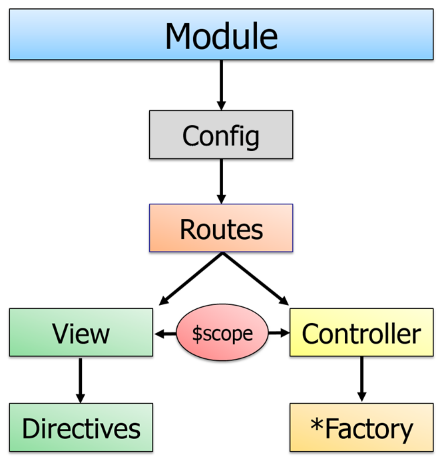
\includegraphics[width=0.5\textwidth]{arqIonic.png}
 \captionsetup{justification=centering,margin=2cm}
 \caption{Arquitectura de Ionic, adoptado para la realizac'ion del proyecto Fuente: \cite{Gallego}}
\label{fig:Ionic}
\end{figure}

Para explicar la arquitectura de ionic se tiene diferentes tipos de componentes, que se explican a continuaci'on:

\begin{enumerate}
\item \textbf{Config y routes:} es el archivo app.js, donde se realiza la configuraci'on y las rutas, que permiten enlazar el controlador con la la interfaz de usuario correspondiente.
\item \textbf{Controller:} es el archivo controller.js,  realiza la comunicaci'on a trav'es de la variable scope entre la interfaz de usuario y los servicios de los archivos services.js o factory.js.
\item \textbf{Directives:} es el archivo directive.js permite crear y usar componentes con aspectos y comportamiento.
\item \textbf{Factory:} son los archivo service.js y factory.js, son modelo de datos que ayudan a obtener los datos, del servicio web.
\item \textbf{View:} son los archivos html que contienen la descripci'on visual y obtiene los datos a mostrar el scope.
\end{enumerate}

\subsection{Estructura del Proyecto}
\label{EstructuraIonic}
El framework ionic, utiliza la estructura de modelo, vista y controlador del proyecto, el c'ual se genera autom'aticamente al momento de crear el proyecto en carpetas y archivos, para organizar el c'odigo en los siguientes archivos:

\begin{verbatim}
 proyecto
    |--bower.json (Lista de dependencias y paquetes de Bower)
    |--.bowerrc
    |--config.xml (Contiene la configuracion de la plataforma)
    |--.editorconfig
    |--.gitignore
    |--gulpfile.js (Lista de tareas de Gulp)
    |--hooks/ (Anade scripts que producen eventos)
    |--ionic.project (Configuracion de Ionic)
    |--package.json (Dependencias y paquetes de NodeJS)
    |--platforms/ (Codigo plataformas para compilar)
    |--plugins/ (Plugins o modulos de aplicacion)
    |--resources/ (Recursos plataforma concreta)
    |--scss/ ( Codigo SCSS compilado en www/css)
    |--www/ (Codigo fuente principal)
        |--css/ (Estilos que se usa en la aplicacion)
        |--img/ (Imagenes de nuestro proyecto)
        |--index.html (Fichero principal, cargamos necesario)
        |--js/ (El codigo, Javascript de la aplicacion)
            |--app.js 
            |--controllers.js
            |--directive.js
            |--factory.js
            |--filter.js
            |--service.js
        |--lib (Librerias, del codigo)
        |--templates/(Vistas de la aplicacion)
\end{verbatim}

\subsection{Configuraci'on del proyecto}

Para, el presente proyecto se utiliza, el interprete de linea de comando denominado (cli) de ionic, el c'ual, tiene los siguientes comandos:

\begin{verbatim}
$ ionic start appSAGAA sidemenu (crea proyecto)
$ ionic platform add android (añadir la plataforma)
$ ionic build android (compilar el proyecto)
$ ionic run android (ejecutar el proyecto)
$ ionic serve (ejecutar, compila y muestra en el navegador )
\end{verbatim}

Se crea autom'aticamente, la carpeta de appSAGAA con  la estructura  de la figura \ref{EstructuraIonic} y el men'u sidemenu por defecto.

\section{Herramientas Extras}
\label{HerramientasExtras}
Para el presente proyecto se ha utilizado algunas herramientas extras como ser: cordova, pouchDB, json web token y localstorage.

\subsection{Framework cordova}
Cordova es un framework de c'odigo libre, para desarrollo m'ovil, que nos permite usar est'andares de tecnolog'ias web como HTML5,CSS3 y Javascript. Se basa en  los enlaces de API's compatibles para acceder a las capacidades del dispositivos como sensores, red, etc. En la figura \ref{fig:arqCordova} se muestra arquitectura de Cordova.

\begin{figure}[H]
\centering
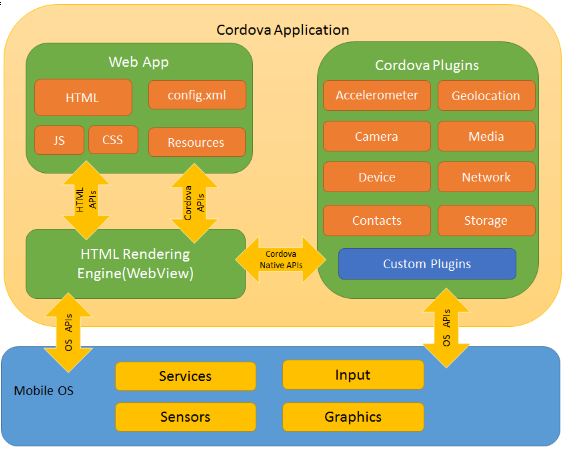
\includegraphics[width=0.3\textwidth]{arqCord.png}
\captionsetup{justification=centering,margin=2cm}
\caption{Arquitectura de Cordova, adoptado para la realizac'ion del proyecto Fuente: \cite{Cantabriatic}}
\label{fig:arqCordova}
\end{figure}

Para el presente proyecto se utiliza cordova, se agrega su librer'ia al proyecto y se instala el plugin necesario.

\subsection{PouchDB}
Es una capa de otras base de datos, se almacenan en el navegador, permite guardar los datos a lado del cliente,  es desarrollado en JavaScript. La estructura de pouchdb, se representa en la figura \ref{fig:pouchDB}. 
\begin{figure}[H]
\centering
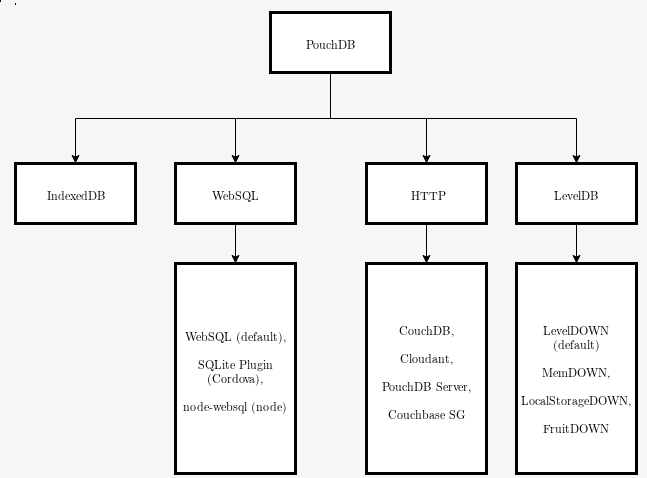
\includegraphics[width=0.3\textwidth]{pouchDB.png}
\captionsetup{justification=centering,margin=2cm}
\caption{Adaptadores de PouchDB, adoptado para la realizac'ion del proyecto Fuente: \cite{Pouch}}
\label{fig:pouchDB}
\end{figure}

Para el presente proyecto se ha utilizado la capa del adaptador de websql, se explica a continuaci'on.
\subsection{Base de datos websql}
Es una herramienta para internet e intranets, facilita el acceso a base de datos relacionada con la web. Integra la tecnolog'ia  del cliente y abre la sybase, el c'ual permite que los datos de la fuente, se han incorporadas din'amicamente en la p'agina web, se representa en la figura \ref{fig:websql}.
\begin{figure}[H]
\centering
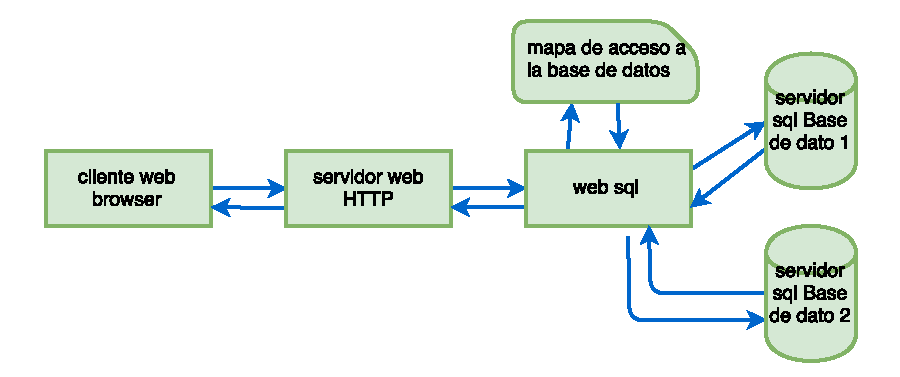
\includegraphics[width=0.6\textwidth]{websql.pdf}
\captionsetup{justification=centering,margin=2cm}
\caption{Base de datos websql, adoptado para la realizac'ion del proyecto Fuente: \cite{Websql1997}}
\label{fig:websql}
\end{figure}

\subsection{Almacenamiento local}
Es una propiedad de HTML5 web de almacenamiento, que permiten almacenar datos en nuestro navegador web denominada localstorage.
Guarda la informaci'on que permanece almacenada por tiempo indefinido, sin importar que el navegador se cierre. Tiene las siguientes caracteristicas, almacenar entre 5MB y 10MB de informaci'on, est'a almacenada en la computadora del cliente y no es enviado en cada petici'on del servidor, previene perdidas de informaci'on cuando se desconecta de la red y la informaci'on es guardada por dominio web \cite{Cardenas2015}.
\subsection{Interceptor}                                                                                                                                                                                                                                              
El interceptor utiliza el servicio de \textit{http}, el c'ual permite la comunicaci'on con el servidor y captura cada petici'on y lo manipula a trav'es del \textit{httpProvider}, es el que registra el contenedor del arreglos y ofrece un servicio regulador.
\subsection{Json web token}
Json web token es un m'etodo abierto y est'andar para representar las  reclamaciones de forma segura, entre dos partes que comparten informaci'on y autentificaci'on moderna, de m'ovil. El c'ual tiene una estructura representada en la figura \ref{fig:jwt}.
\begin{figure}[H]
\centering
\includegraphics[width=0.6\textwidth]{jwt.pdf}
\captionsetup{justification=centering,margin=2cm}
\caption{Json web token, adoptado para la realizac'ion del proyecto Fuente: Elaboraci'on propia}
\label{fig:jwt}
\end{figure}

Estos son las herramientas extras, se utilizan para el presente proyecto, los c'uales son compatibles con el framework ionic.

\section{Implementaci'on del Proyecto}
Para la implementaci'on del presente proyecto, se ha utilizado las herramientas \ref{HerramientaMovil} y las herramientas extras \ref{HerramientasExtras}, se ha realizado seg'un los modulos \ref{ModuloMovil}, el dise'no de interfaz \ref{DisenoMovil} que se han realizado en el c'apitulo \ref{capituloseis}
dividido en los siguientes intento.

\subsection{El primer intento o iteraci'on la configuraci'on para conectarse al servicio web}
Configurar la aplicaci'on m'ovil para solicitar la planilla de notas al servicio web, se explican los puntos importantes:

\begin{enumerate}
\item La configuraci'on para conectar la aplicaci'on m'ovil al servicio web, se realizo en el archivo www/js/fileFactory.js: 
\begin{verbatim}
//IP de la maquina donde se encuentra el server.js
var urlBase = 'http://172.20.10.3:8080';
var conf = {
	headers : {
	'Access-Control-Allow-Origin' : '*',
    'Access-Control-Allow-Methods' : 'POST, GET, OPTIONS, PUT',
    'Content-Type': 'application/jsonr',
    'Accept': 'application/json'
    } 
};
\end{verbatim}

\item Solicitud de la planilla de notas al servicio web, se realizo en el archivo www/js/fileFactory.js

\begin{verbatim}
sisFactory.posDataDetalle = function(carrera){
.......
 $http.post(urlBase+'/detalle', descargarD, {skipAuthorization : false}, conf).
 success(function(data) {
 .......
 }; 
\end{verbatim}

\item Ordenar los datos del servicio web, se realizo en el archivo www/js/fileService.js.

\begin{verbatim}
divFile : function(data , template){
if(template == 'informacion'){
   	return (((((data.pcd).head)[0]).info))[0];
	.........
},
crearBDInf : function(array){
	return  newBD = {
    	'fechaC ' : array[0],
        'fecgaE'  : array[1],
        'codDoc' : array[2],
        'nomApeDoc' : array [3],
        ..........
    };
},
\end{verbatim}
\end{enumerate}
\subsection{El segundo intento o iteraci'on la sesi'on}
Para asegurar la sesi'on el servicio web, 'envia en la cabecera la llave denominado jwt, el c'ual se explica la implementaci'on en las partes importante a continuaci'on:
\begin{enumerate}
\item La configuraci'on para enviar el jwt en la cabecera de la petici'on, se crea el interceptor, el c'ual se guarda localmente, se realizo en el archivo www/app.js

\begin{verbatim}
...
.config(function($stateProvider, $urlRouterProvider, $authProvider, 
$httpProvider, jwtInterceptorProvider, jwtOptionsProvider) { 
.....
 jwtOptionsProvider.config({
 	//IP de la maquina actual 
	 whiteListedDomains: ['localhost', '172.20.10.3'] 
	 tokenGetter: function(options, jwtHelper){
	 var token = localStorage.getItem('id_token');
}});
	//metodo para enviar un json web token
$httpProvider.interceptors.push('jwtInterceptor');
......
\end{verbatim}
\end{enumerate}

\subsection{El tercer intento o iteraci'on trabajar sin el servicio web}
Para modificar la planilla de notas, sin conexi'on a internet, anteriormente ha debido crear su sesi'on y descargar la planilla que utilizan localmente, se muestra los puntos mas importantes:
\begin{enumerate}
\item Se utiliza el pouchdb y websql para crear, actualizar y modificar la base de datos, se realizo en el archivo www/js/fileService.js.
\begin{verbatim}
.service('SagaaService', function($q) {
......
_db = new PouchDB('sagaa', { adapter: 'websql' }, 
 { skip_setup: true });//crear base de datos
 ......
  return $q.when( _db.post( sagaa));//añadir
  ......
  return $q.when(_db.put(sagaa));//actualizar
   .......
\end{verbatim}
\item Se guardan las solicitudes al servicio web, que tienen alg'un problema con la conecci'on, se realizo en el archivo app.js.
\begin{verbatim}
.....
//crea un interceptor
$httpProvider.interceptors.push('myInterceptor');
.....
//crear un interceptor
//crear metodo, para conocer la respuesta o la peticion
var interceptor = function ($q, logHttp) {
return {
  responseError: function(rejection) {
  logHttp.push(rejection.config);
  ......
  return $q.reject(rejection);
  ......}
}
\end{verbatim}
\item Guardar y verificar las peticiones, se realizo en el fileService.js  
\begin{verbatim}
.service('myInterceptor', function($q, $timeout, logHttp){
return { 
	'request': function(config){ 
	......//guardamos la peticion sin error
	logHttp.push(config);
	.....
	'requestError': function(rejection){
	//guarda la peticion con error, 
	window.localStorage.setItem('id_request', data);
	......// lo mismo realiza en la respuesta con error
	.......
.service('logHttp', function($q) {
	push: function(config) {
	requestsConfig = config;
.............
\end{verbatim}
\end{enumerate}
